\section{Durchf\"uhrung}

In  diesem Versuch werden zwei verschiedene Materialien (Teppich und Platik) mit
konstanter   (einstellbarer)   Geschwindigkeit   \"uber   eine   Gleitbahn   von
$\approx\SI{2}{\meter}$ gezogen.  Ein  geregelter Motor treibt ein Schlepper an,
der  eingebaut  ein  Biegebalken-Kraftmesser hat, damit die Reibungskraft direkt
gemessen werden kann.

Die Bahn ist horizontal, was heisst dass die  Normalkraft  gleich  ist  wie  die
Gewichtskraft.

\begin{figure}[H]
    \centering
    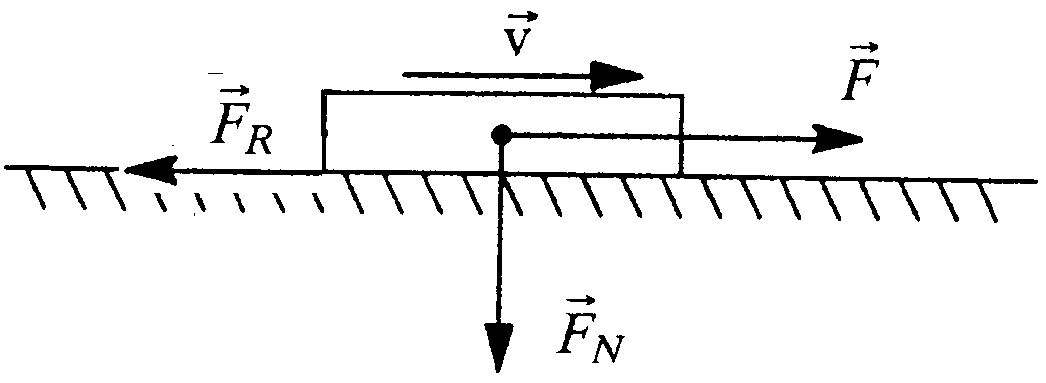
\includegraphics[width=.7\linewidth]{images/reibungskraefte}
    \caption{}
\end{figure}


\subsection{Kalibrationsmessung}

F\"ur  die  Kalibrationsmessung wurde ein Faden an den  Kraftsensor  angebracht,
\"uber ein Rad gespannt und  verschiedene  Normgewichte  wurden  am anderen Ende
angeh\"angt.  Der  Aufbau   ist   in   Abbildung   \ref{fig:kalibration_aufbau}.

\begin{figure}[H]
    \centering
    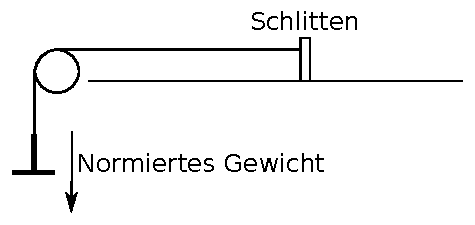
\includegraphics[width=.6\linewidth]{images/kalibration_aufbau}
    \caption{Aufbau der Gewichts-Kalibrationsmessung.}
    \label{fig:kalibration_aufbau}
\end{figure}

Die  Geschwindigkeit  des  Schlittens musste auch kalibriert werden. Dabei wurde
der  Schlitten  bei  verschiedenen  einstellungen  des  Potentiometers  zeitlich
gemessen, um zu sehen, wie lange sie braucht, um eine Strecke von \SI{1}{\meter}
zur\"uckzulegen. Diese Messung wurde mit  einer  Stoppuhr und einem auf der Bahn
angebrachten Massstabe durchgef\"uhrt.


\subsection{Gleitreibungskraft}

Ein  \SI{1}{\kilo\gram}  wiegendes  Objekt  wurde  einerseits bei  verschiedenen
Geschwindigkeiten   und   konstantem  Gewicht,  anderseits   mit   verschiedenen
Zusatzgewichten  und  konstanter  Geschwindigkeit  \"uber  die   Bahn   gezogen.

Das  Objekt  ist  ein  Klotz  der  aus  Holz  besteht. Auf einer Seite  ist  ein
Teppichausschnitt angebracht, auf  der anderen Seite ist Plastik angebracht. Die
beiden Materialien k\"onnen also getestet werden indem der Klotz umgedreht wird.

In der Abbildung \ref{fig:messaufbau} ist der Messaufbau zu sehen.

\begin{figure}[H]
    \centering
    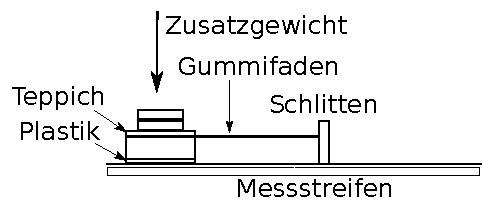
\includegraphics[width=.6\linewidth]{images/messaufbau}
    \caption{Aufbau f\"ur beide Messungen}
    \label{fig:messaufbau}
\end{figure}

